% This file was created by tikzplotlib v0.9.8.
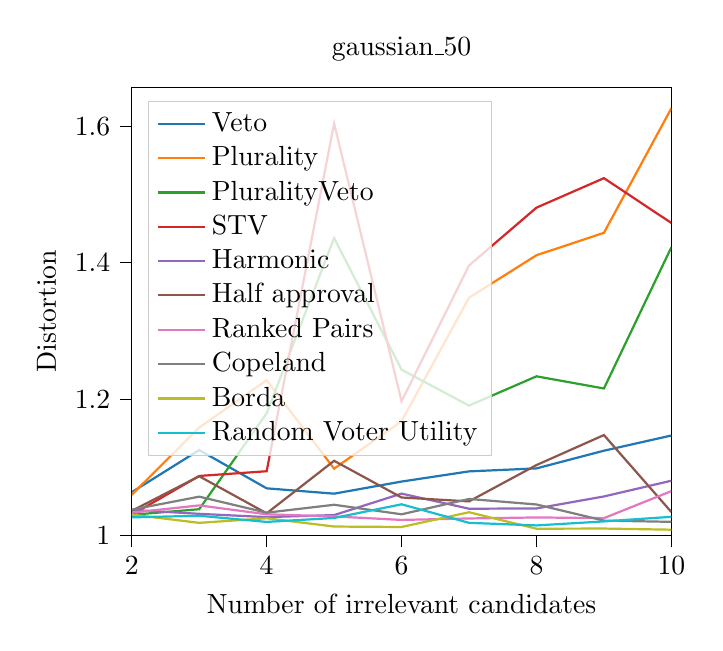
\begin{tikzpicture}

\definecolor{color0}{rgb}{0.12156862745098,0.466666666666667,0.705882352941177}
\definecolor{color1}{rgb}{1,0.498039215686275,0.0549019607843137}
\definecolor{color2}{rgb}{0.172549019607843,0.627450980392157,0.172549019607843}
\definecolor{color3}{rgb}{0.83921568627451,0.152941176470588,0.156862745098039}
\definecolor{color4}{rgb}{0.580392156862745,0.403921568627451,0.741176470588235}
\definecolor{color5}{rgb}{0.549019607843137,0.337254901960784,0.294117647058824}
\definecolor{color6}{rgb}{0.890196078431372,0.466666666666667,0.76078431372549}
\definecolor{color7}{rgb}{0.737254901960784,0.741176470588235,0.133333333333333}
\definecolor{color8}{rgb}{0.0901960784313725,0.745098039215686,0.811764705882353}

\begin{axis}[
legend cell align={left},
legend style={
  fill opacity=0.8,
  draw opacity=1,
  text opacity=1,
  at={(0.03,0.97)},
  anchor=north west,
  draw=white!80!black
},
tick align=outside,
tick pos=left,
title={gaussian\_50},
x grid style={white!69.0196078431373!black},
xlabel={Number of irrelevant candidates},
xmin=2, xmax=10,
xtick style={color=black},
y grid style={white!69.0196078431373!black},
ylabel={Distortion},
ymin=1, ymax=1.65759797067672,
ytick style={color=black}
]
\addplot [thick, color0]
table {%
2 1.06345233430277
3 1.12526202730556
4 1.06913251799567
5 1.06130933004343
6 1.07907054193565
7 1.09399099697435
8 1.09838498403126
9 1.12433208914125
10 1.14662575133231
};
\addlegendentry{Veto}
\addplot [thick, color1]
table {%
2 1.05969835409312
3 1.15827664366635
4 1.2278465105087
5 1.09800458620337
6 1.16758980848519
7 1.34870663645928
8 1.41101393118544
9 1.44395645377376
10 1.62668672413809
};
\addlegendentry{Plurality}
\addplot [thick, color2]
table {%
2 1.03029604880687
3 1.0385192656154
4 1.17917173956267
5 1.43633228253004
6 1.24312912164117
7 1.19047646385083
8 1.23342443475536
9 1.21557901543272
10 1.4228139648318
};
\addlegendentry{PluralityVeto}
\addplot [thick, color3]
table {%
2 1.03032418958142
3 1.08728887258623
4 1.09422028172221
5 1.60430475871517
6 1.19677614923991
7 1.39606243171255
8 1.48083241518552
9 1.52409838168211
10 1.45832832254617
};
\addlegendentry{STV}
\addplot [thick, color4]
table {%
2 1.03747975476663
3 1.03173208888521
4 1.02692452374335
5 1.02989666158134
6 1.06140867672463
7 1.03921713602047
8 1.03963310756812
9 1.05721088008193
10 1.08031483820393
};
\addlegendentry{Harmonic}
\addplot [thick, color5]
table {%
2 1.03607581813205
3 1.08687727344591
4 1.03245868970609
5 1.10952377639007
6 1.05568687977795
7 1.04997833170272
8 1.10327105920941
9 1.1472634225823
10 1.03430687311724
};
\addlegendentry{Half approval}
\addplot [thick, color6]
table {%
2 1.0334207643677
3 1.04409163436096
4 1.0310521875604
5 1.02794396360091
6 1.02278388577861
7 1.02493103750951
8 1.02643279976712
9 1.02540367664131
10 1.06507550593552
};
\addlegendentry{Ranked Pairs}
\addplot [thick, white!49.8039215686275!black]
table {%
2 1.03784685183929
3 1.05691936202676
4 1.03340559607788
5 1.04502144762768
6 1.03105540243719
7 1.05352761615107
8 1.04546701172244
9 1.02176699078613
10 1.01998205542995
};
\addlegendentry{Copeland}
\addplot [thick, color7]
table {%
2 1.03058077726297
3 1.0184812582161
4 1.02522255217816
5 1.01307693709507
6 1.01244443116972
7 1.03405977170773
8 1.00992058867186
9 1.01012695192175
10 1.00846179336547
};
\addlegendentry{Borda}
\addplot [thick, color8]
table {%
2 1.0265482275272
3 1.02891370854817
4 1.01988218784486
5 1.02565644797148
6 1.04569706559287
7 1.01853576882013
8 1.01472892629021
9 1.02060834887079
10 1.02737040032201
};
\addlegendentry{Random Voter Utility}
\end{axis}

\end{tikzpicture}
